\chapter{Advanced Process Discovery: Dependency Measure, Causal Nets, and Heuristic Miner}
To improve our Petri net models, we need to address certain limitations. Initially, we notice several problems:
\begin{itemize}
    \item The current notation does not capture the \textbf{frequency} of events, which means it treats rare events the same as frequent ones.
    \item There is no clear distinction between \textbf{causal relationships}, such as AND splits and XOR splits, in the coverability graph.
\end{itemize}
To address these issues, we introduce the \textbf{dependency measure}, which allows us to quantify the dependency between activities and account for noise.

\section{Dependency Measure}

The \textbf{dependency measure} quantifies the strength of the dependency between two activities \(a\) and \(b\). The formula is as follows:
\begin{equation}
    |a \Rightarrow_L b| =
\begin{cases}
\frac{|a >_L b| - |b >_L a|}{|a >_L b| + |b >_L a| + 1} \hspace{3mm} a \neq b \\
\frac{|a >_L a|}{|a >_L a|+1} \hspace{3mm} a = b
\end{cases}
\end{equation}

Where:
\begin{itemize}
    \item \(|a >_L b|\) represents the number of times \(a\) is directly followed by \(b\),
    \item \(|b >_L a|\) represents the number of times \(b\) is directly followed by \(a\),
    \item The addition of \(+1\) in the denominator prevents division by zero in cases where there is no relationship between \(a\) and \(b\).
\end{itemize}

This measure ranges from \(-1\) to \(1\), where:
\begin{itemize}
    \item If \(|a >_L b| \gg |b >_L a|\), then \(a \Rightarrow_L b \approx 1\), indicating a strong causal relationship.
    \item If \(|a >_L b| = |b >_L a|\), then \(a \Rightarrow_L b = 0\), meaning no clear dependency.
    \item If \(|b >_L a| \gg |a >_L b|\), then \(a \Rightarrow_L b \approx -1\), indicating reverse causality.
\end{itemize}

The dependency measure also filters out noise, as arcs with low dependency values are considered less relevant.

\section{Causal Nets (C-nets)}

To further address the limitations of Petri nets, we introduce \textbf{Causal nets (C-nets)}. C-nets are more expressive and allow us to explicitly model how transitions occur. In a C-net, every activity requires an \textbf{obligation} (similar to tokens) for activation. Once activated, the activity consumes its input obligations and produces new ones for subsequent activities.

\begin{center}
    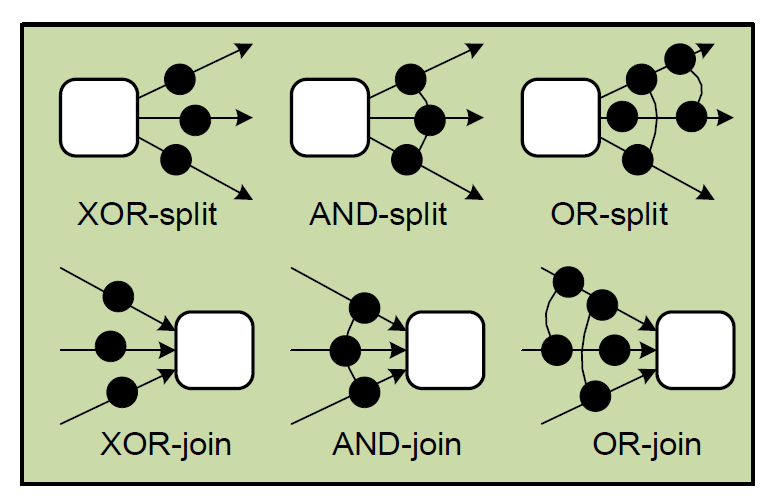
\includegraphics[width=0.5\textwidth]{capitolo 6/6 cnet notation.png} % Insert image of Causal Net patterns
\end{center}

\subsection{Binding Obligations}
In C-nets, obligations work similarly to tokens in Petri nets. When an activity is activated, it "burns" its input obligations and generates new output obligations, as shown below:

\begin{center}
    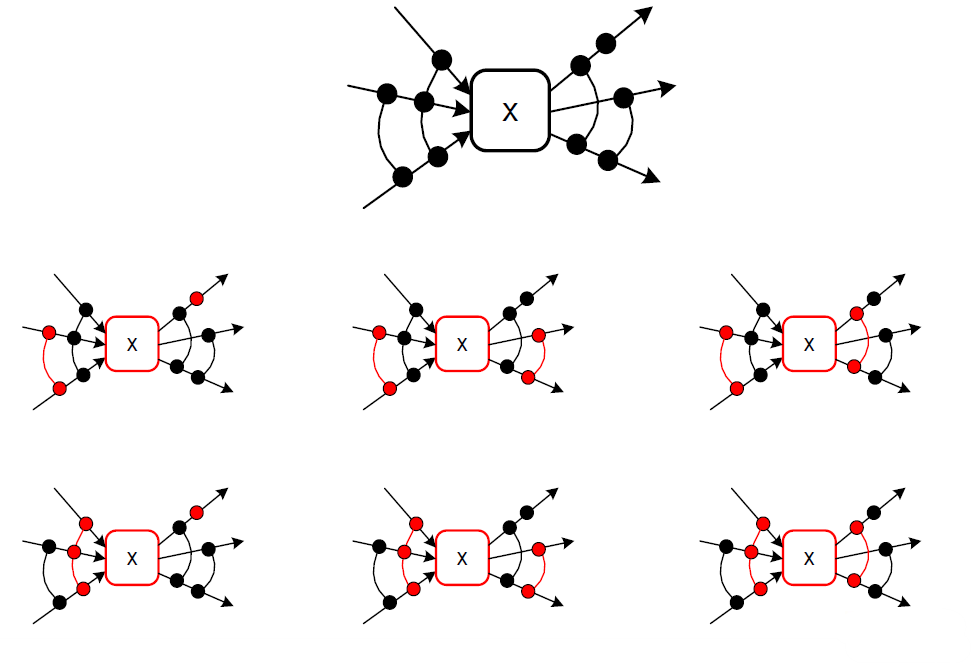
\includegraphics[width=0.5\textwidth]{capitolo 6/6 binding.png} % Insert image of binding example
\end{center}

From any Causal net, it is possible to derive a Petri net, and vice versa. Each \textbf{invisible transition} in the Petri net can be treated as a different binding in the C-net.

\begin{center}
    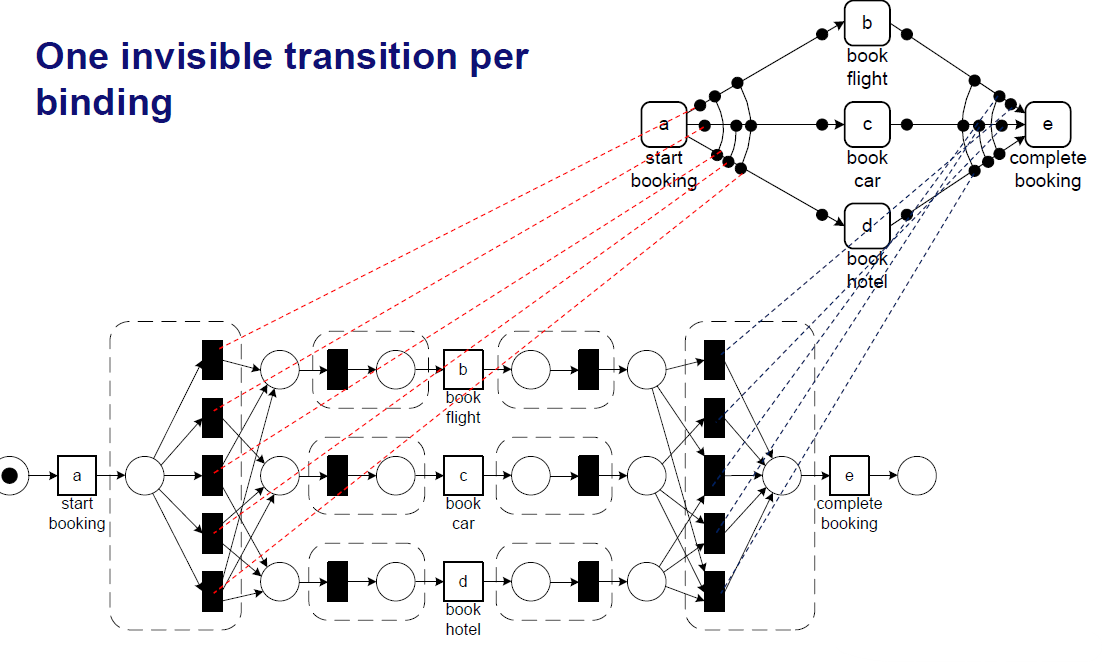
\includegraphics[width=0.8\textwidth]{capitolo 6/6 cnet to petri.png} % Insert image showing conversion from C-net to Petri net
\end{center}

However, the C-net model is not yet perfect and might not always be sound.

\section{Heuristic Miner}

The \textbf{Heuristic Miner} introduces a different approach. Instead of solely focusing on direct causality, it considers the frequency of activities. The steps are:
\begin{enumerate}
    \item Given an event log, build a \textbf{dependency graph}.
    \item Learn where the splits and joins are (AND/XOR).
    \item Visualize them and provide the graph to a tool.
    \item The tool counts how often certain sets of inputs and outputs appear, allowing it to calculate the frequency of bindings and select the most frequent ones.
\end{enumerate}

The \textbf{best guess} approach is used, meaning the miner does not analyze end-to-end traces but rather makes decisions based on local observations.

\subsection{Example: Infinite Window}
Let's explain the process of constructing initial and final bindings using the infinite window approach. In this example:
\begin{center}
    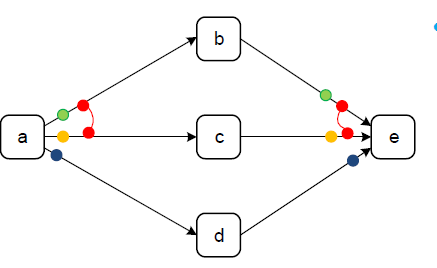
\includegraphics[width=0.5\textwidth]{capitolo 6/6 infinite window.png} % Insert image for Infinite Window example
\end{center}

\begin{itemize}
    \item Activity \(A\) is sometimes followed by \(B\) and \(C\) but not by \(D\). This occurs in the traces \(\langle a, b, c, e \rangle\) and \(\langle a, c, b, e \rangle\).
    \item Therefore, this suggests an \textbf{AND-split} of \(A\) with \(B\) and \(C\) (red dots).
    \item Activity \(A\) is sometimes followed by only \(E\), as seen in the trace \(\langle a, e \rangle\). However, this is ignored as there is no significant dependency. 
    \item Activity \(A\) is sometimes followed by \(B\) but not by \(C\) or \(D\), as shown in the trace \(\langle a, b, e \rangle\) (green dot).
    \item Activity \(A\) is sometimes followed by \(C\) but not by \(B\) or \(D\), as shown in the trace \(\langle a, c, e \rangle\) (yellow dot).
    \item Finally, \(A\) is sometimes followed by \(D\) but not by \(B\) or \(C\), in traces like \(\langle a, d, ..., d, e \rangle\) (blue dot).
\end{itemize}

This results in the following structure:
\[
A \rightarrow B, C, D
\]

In this example, we focus on how activity \(E\) behaves:
\begin{itemize}
    \item Activity \(E\) is sometimes preceded by \(B\) and \(C\) but not by \(D\), as in the traces \(\langle a, b, c, e \rangle\) and \(\langle a, c, d, e \rangle\), indicating an \textbf{OR-join} with \(B\) and \(C\) (red dots).
    \item Sometimes \(E\) is preceded only by \(A\), as in \(\langle a, e \rangle\), which is ignored due to lack of dependency.
    \item \(E\) is also preceded by \(B\) but not by \(C\) or \(D\), as seen in \(\langle a, b, e \rangle\) (green dot).
    \item Similarly, \(E\) is preceded by \(C\) but not by \(B\) or \(D\), as in \(\langle a, c, e \rangle\) (yellow dot).
    \item Finally, \(E\) is preceded by \(D\) but not by \(B\) or \(C\), in traces like \(\langle a, d, ..., d, e \rangle\) (blue dot).
\end{itemize}

This produces the structure:
\[
E \rightarrow B, C, D
\]



\section{Region Miner (use slides for better images)}

Another advanced model is the \textbf{Region Miner}. The goal is to learn a transition system from an event log using state abstraction, then transform it into a Petri net.

The \textbf{transition system} allows us to understand the past and future of a given state. We use a schema, represented by black dots, to abstract states.

\begin{center}
    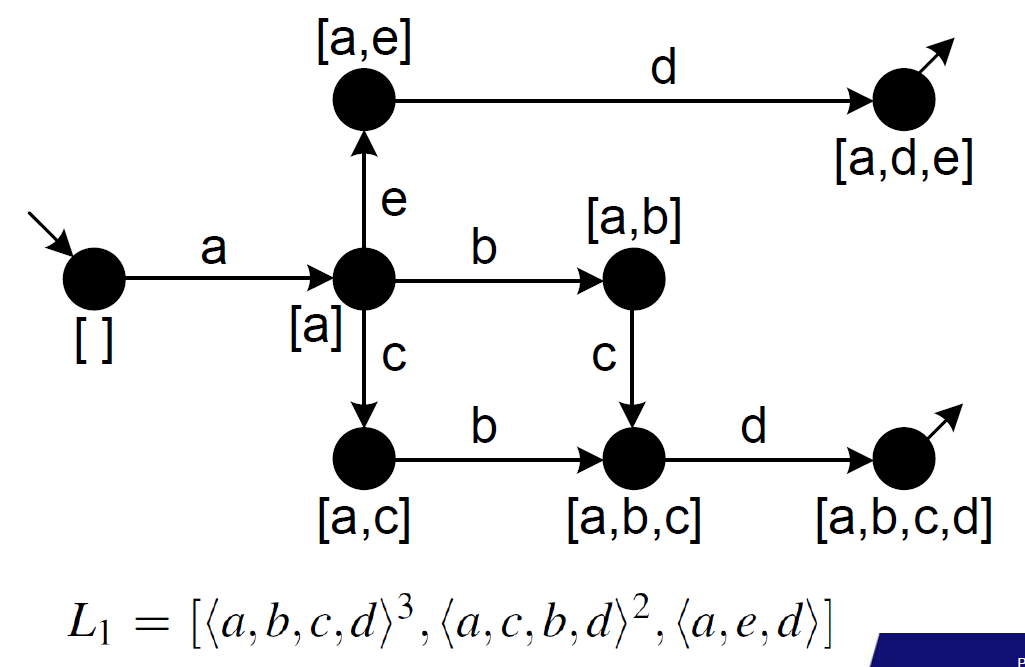
\includegraphics[width=0.5\textwidth]{capitolo 6/6 region miner scheme.png} % Insert image showing transition system abstraction
\end{center}

From the transition system, we can move to a Petri net by delimiting regions. A \textbf{region} corresponds to a place in the Petri net. A region is a set of states such that:
\begin{itemize}
    \item If a transition exits the region, then all transitions with the same label exit the region.
    \item If a transition enters the region, then all transitions with the same label enter the region.
    \item Events that do not enter or exit the region do not cross it.
\end{itemize}

\begin{center}
    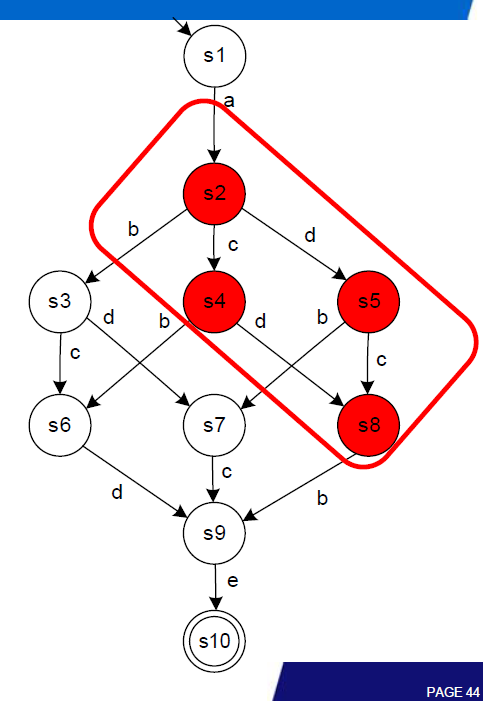
\includegraphics[width=0.5\textwidth]{capitolo 6/6 region 1.png} % Insert image showing region definition
\end{center}

\subsection{Minimal Regions}
We aim to extract the \textbf{minimal regions}, which are regions that do not contain other regions within them. Additionally:
\begin{itemize}
    \item The set \(S\) of all states and the empty set are \textbf{trivial regions}.
    \item If \(r\) is a region, then \(S \setminus r\) is also a region.
    \item If \(r_0\) and \(r_1\) are regions, and \(r_0 \subseteq r_1\), then \(r_1 \setminus r_0\) is a region.
\end{itemize}

\begin{center}
    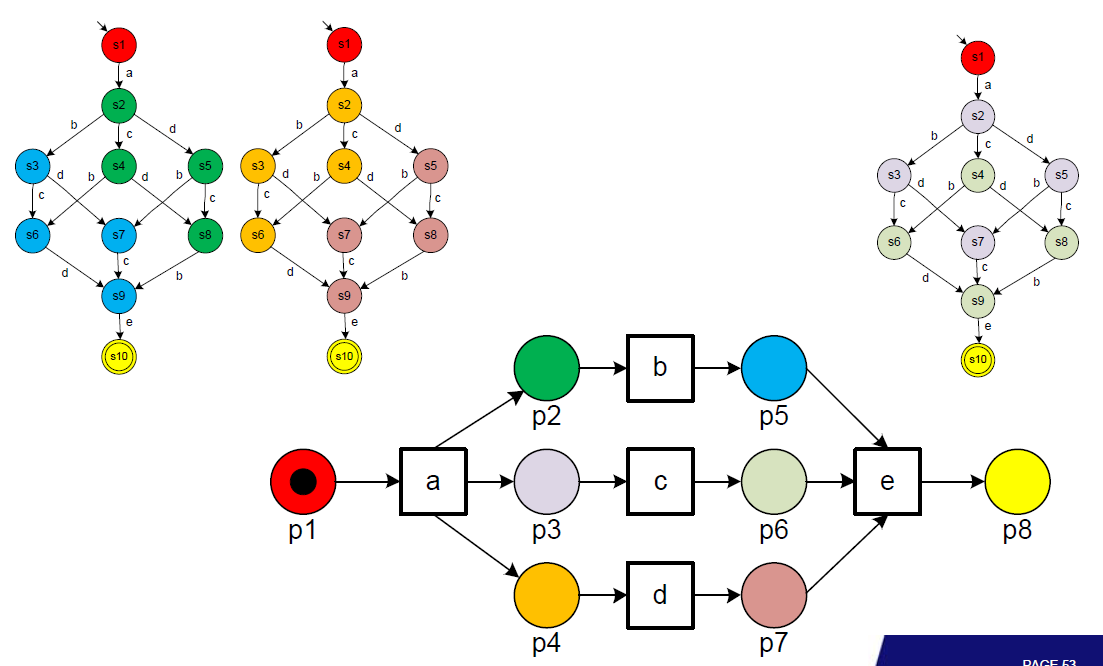
\includegraphics[width=0.8\textwidth]{capitolo 6/6 region 2.png} % Insert image showing minimal region example
\end{center}

\section{Algorithm for Constructing a Petri Net from a Transition System}

The algorithm to generate a Petri net from a transition system is as follows:
\begin{enumerate}
    \item For each event in the transition system, generate a transition in the Petri net.
    \item Compute the minimal non-trivial regions.
    \item For each minimal region, generate a place in the Petri net.
    \item Add corresponding arcs: post-regions as output places and pre-regions as input places.
    \item Add tokens to places that correspond to regions containing the initial state.
\end{enumerate}

\section{Conclusion}
Through advanced process discovery techniques like dependency measures, Causal nets, and region miners, we can construct more refined process models that account for frequency, noise, and complex dependencies. However, challenges like soundness and overfitting remain, and the selection of the appropriate discovery method depends on the specific use case.


